\section{Store Consistency}
\label{sec:store-consistency}

Under a trivial trace invariant (i.e., $\I(\E) = true$), the abstract
machine of Fig.~\ref{fig:txnimp} assumes the semantics of an {\sc ec} store;
it allows operations of a transaction to witness arbitrary subsets of the
global state. A non-trivial $\I$ composed of isolation specifications
from Fig.~\ref{fig:ansi-isolation} induces the machine to provide
non-trivial isolation guarantees for transactions. However, weak
isolation levels often only constrain the visibility sets of
operations by dictating what \emph{not} to see; not what to see.  For
instance, \iso{Repeatable Read} isolation prohibits operations of a
transaction from witnessing different states. It, however, does not
prohibit all operations of a transaction from witnessing an aribitrary
subset of the global state. Consequently, the machine can remain an {\sc ec}
store even while providing non-trivial isolation. How then to model
the semantics of an {\sc sc} store, such as a relational database, with
variable (weak) isolation?

The answer lies in enforcing store-specific consistency constraints,
along with transaction-specific isolation constraints, via the trace
invariant $\I$. In particular, we split $\I$ into two components: (1).
$\I_s$, the store-specific invariant, and (2). $\I_c$, the
program-specific (or, client-specific) invariant, to capture
consistency and isolation constraints, respectively. $\I$ is now a
conjunction:
\begin{smathpar}
  \I \;=\; \lambda\E.~\I_s(\E) \wedge \I_c(\E)
\end{smathpar}
The trace invariant defined in \S\ref{sec:ansi-isolation} for the
withdraw program of Fig.~\ref{fig:motiv-eg-1} now becomes its $\I_c$
and remains an invariant regardless of the store. $\I_s$ however
changes from store to store. We now consider various stores and
describe their corresponding store invariants.

\paragraph{An EC store} An eventually-consistent {\sc ec} store provides no
additional consistency guarantees besides those provided by the operational
semantics.  Hence, its trace invariant, $\I_s(\E)$, for any execution
$\E$ is always \emph{true}.

\paragraph{An SC store} A strongly-consistent {\sc sc} store guarantees a total order of
all operations w.r.t $\visZ$ consistent with their chronological
order. A straightforward definition of $\I_s$ for this store is:
\begin{smathpar}
\begin{array}{l}
  \C{SC}(\E) \;=\; \forall\eta_1,\eta_2.~\{\eta_1,\eta_2\}
  \subseteq \E.\A \conj \id(\eta_1) < \id(\eta_2) \\
  \hspace*{2in}\Rightarrow \underE{\eta_1 \visar \eta_2}
\end{array}
\end{smathpar}
Unfortunately, $\I_s=\C{SC}$ conflicts with all isolation
specifications of Fig.~\ref{fig:ansi-isolation}. For instance,
consider a case where $\I_c(\E) \;=\; \forall
T_i.~\underE{\C{RC}(T_i)}$, a constraint that dictates all transactions execute under
\iso{Read Committed} isolation. Imagine a sample execution where
$\eta_1$'s transaction is not yet committed when $\eta_2$ is
generated. Letting $\eta_1$ be visible to $\eta_2$ violates $\I_c$,
whereas not letting it be visible violates $\I_{s}$. The only way to
satisfy both the invariants is to rule out all the executions that
interleave the operations of one transaction with the other, thereby
enforcing serializability and the ACID model of
transactions\footnote{Thus, serializability is a natural
generalization of {\sc sc} to transactions.}. In general, when $\I_s$ is in
conflict (but not inconsistent) with $\I_c$, the only way to enforce
both invariant sets is to restrict concurrency. Clearly, this is unacceptable since
it defeats the very purpose of supporting weak isolation. 
% How then do we enforce weak isolation on a strongly consistent
% machine?

Relational databases demonstrate a way of out this impasse.
Implementations of weak isolation levels on relational databases
implicitly relax the {\sc sc} requirement so as to maximize
concurrency and improve performance. Consequently, execution traces do
not necessarily satisfy {\sc sc}. This approach hints at a general
solution reconciling $\I_s$ with $\I_c$ that entails weakening the
former sufficiently to satisfy the latter. However, there are many
ways $\I_s$ can be weakened; for instance, by setting it to \emph{true}
which makes the store EC. In reality though, weak isolation on
databases does not cause so drastic a reduction in consistency. It is
therefore possible that there exists a principled approach to weaken
$\I_s$ that adequately captures the underlying properties provided by the store. Such
a principle can be gleaned by observing that data stores often make
\emph{recency} commitments~\cite{bailishat}, by which they aim to make
the most recent data available to clients; {\sc sc} is, in fact, an
extreme form of a recency commitment, which guarantees that reads
\emph{always} witness the most recent writes to a data item. In case this conflicts
with weak isolation guarantees, such as {\sc rr} which only requires that
reads in a transaction witness the same state, the natural way to
weaken consistency while prioritizing recency is to let reads witness
the most recent state that \emph{does not} violate isolation
constraints. In the context of the operational model of
Fig.~\ref{fig:txnimp}, this translates to making the largest subset
($S$) of the global state ($\A$) that does not lead to the violation
of {\sc rr} isolation constraints visible to an operation.

Generalizing this intuition to any $\I_s$ and $\I_c$ yields a
\emph{maximum visiblity principle}, which requires the weakened
consistency guarantee ($\I_s'$) of a store to enforce all visibility
relationships imposed by the actual consistency guarantee ($\I_s$) on
a given trace, unless enforcing such a relationship violates $\I_c$.
Formally, the maximum visibility weakening of $\I_s$ is a new store
consistency relation $\I_s'$, such that:
\begin{itemize}
  \item $\I_s'$ is weaker than $\I_s$: 
      $\forall\E.~ \I_s(\E) \Rightarrow \I_s'(\E)$, and
  \item In every trace $\E$ that satisfies $\I_c$, and for every pair
  of effects $\eta_1$ and $\eta_2$ in $\E$, if $\I_s(\E)$ requires
  $\eta_1$ to be visible to $\eta_2$, then so does $\I_s'(\E)$ unless
  extending $\E$ with $\visZ(\eta_1,\eta_2)$ violates
  $\I_c$\footnote{\GK{ToDo: consider other well-formedness conditions
  on trace, such as acyclicity of $\visZ$ and $\soZ$. Are they needed
  (considering that the machine never violates them)? Encode the
  specifications in Z3 and make sure they are consistent.}}:
  \begin{smathpar}
  \begin{array}{l}
  \forall\E,\eta_1,\eta_2.~ \I_c(\E) \Rightarrow (\I_s(\E)
    \Rightarrow \underE{\eta_1 \visar \eta_2}) \Rightarrow \\
    \hspace*{0.5in}(\I_s'(\E) \Rightarrow \underE{\eta_1 \visar
    \eta_2} \disj \neg\I_c(\E\,\cup\,(\emptyset,\{(\eta_1,\eta_2)\})))
  \end{array}
  \end{smathpar}
\end{itemize}

Applying this principle, we can weaken {\sc sc} to obtain the
following store trace invariant ($\I_s$) for an {\sc sc} store whose
isolation constraints are captured by $\I_c$:

\begin{smathpar}
\begin{array}{lcl}
\I_s(\E) & = & \forall \eta_1,\eta_2.\, \{\eta_1,\eta_2\},
    \subseteq \E.\A \conj \id(\eta_1) <
    \id(\eta_2) \\
    & & \hspace*{0.5in} \Rightarrow 
      \underE{\eta_1 \visar \eta_2} \disj \neg\I_c(\E
    \cup (\emptyset,\{(\eta_1,\eta_2)\}))\\
\end{array}
\end{smathpar}

\noindent As usual $\I = \I_s \wedge \I_c$. The resultant operational model
hides an existing effect ($\eta\in\A$) from being visible to the
current operation if and only if showing it results in the violation
of $\I_c$.

It is worthwhile to note that although the conflict-free definition of
$\I_s$ shown above captures the behaviour of an {\sc sc} database in
the presence of isolation constraints, it does not necessarily describe
how the database achieves this behaviour (i.e., its
implementation). It is unusual for databases to check for satisfaction
of isolation constraints every time an operation is executed. Efficient
implementation strategies (\eg multi-versioning) are employed to
achieve the twin goals of isolation and consistency/recency. \footnote{\SJ{This
  paragraph reads poorly - not quite sure what the reader should conclude
  from this.  A negative interpretation is that we can formalize the
  relationship between $I_s$ and $I_c$ but the formalization may be
  far removed from reality and practicality.}}

\paragraph{A CC store} A causally consistent data store~\cite{gotsmanpopl16,LBC16}
allows operations to only witness a causally consistent snapshot of the
global state. A straightforward trace invariant ($\I_s$) for this
store is the causally consistent guarantee that requires an effect to witness all
causally preceding effects regardless of the isolation requirements of
its transaction:
\begin{smathpar}
\begin{array}{lccl}
\C{CC}(\E) & \;=\; &  & \forall \eta_1,\eta_2.\, 
      \E \Vdash \eta_1 \soar \eta_2 \Rightarrow  \underE{\eta_1 \visar
      \eta_2}\\
    &   & \wedge & \forall\eta_1,\eta_2,\eta_3.\,\underE{\eta_1 \visar
      \eta_2} \conj \underE{\eta_2 \visoar \eta_3} \\
    &   & &\hspace*{0.5in} \Rightarrow \underE{\eta_1 \visar \eta_3}\\
\end{array}
\end{smathpar}
In order to admit weak isolation behavior without restricting concurrency, we weaken $\I_s$ while
being guided by the maximum visibility principle. The weakened $\I_s$
is shown below:

\begin{smathpar}
\begin{array}{lccl}
\C{CC}(\E) & \;=\; &  & \forall \eta_1,\eta_2.\, 
      \E \Vdash \eta_1 \soar \eta_2 \Rightarrow  \underE{\eta_1 \visar
      \eta_2} \\
    & & & \hspace*{0.6in}\disj \neg\I_c(\E \cup 
                (\emptyset,\{(\eta_1,\eta_2)\}))\\
    &   & \wedge & \forall\eta_1,\eta_2,\eta_3.\,\underE{\eta_1 \visar
      \eta_2} \conj \underE{\eta_2 \visoar \eta_3} \\
    &   & &\hspace*{0.3in} \Rightarrow \underE{\eta_1 \visar \eta_3}
      \disj \neg\I_c(\E \cup (\emptyset,\{(\eta_1,\eta_2)\}))\\
\end{array}
\end{smathpar}

\noindent Instantiating the parameter $\I$  with $\I_s \wedge \I_c$ in
Fig.~\ref{fig:txnimp} results in an operational semantics that admits
violation of causal consistency if and only if the violation is
inevitable to enforce $\I_c$.

\subsection{Eventually Consistent Replication}

\begin{figure}
\centering
\subcaptionbox {
  Replica model
  \label{fig:ec-theirs}
} [
  0.4\columnwidth
] {
  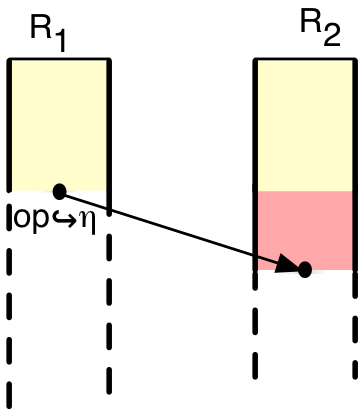
\includegraphics[scale=0.7]{Figures/ec-theirs}
 
}
\hspace*{0.1in}
\subcaptionbox {
  Subset model
  \label{fig:ec-ours}
}{
  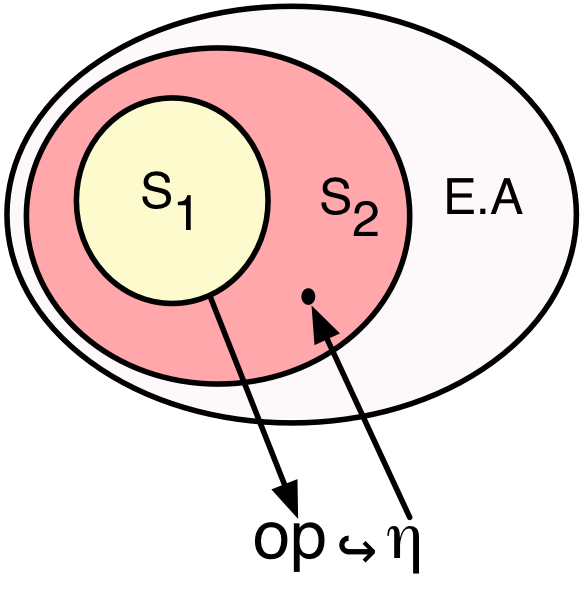
\includegraphics[scale=0.45]{Figures/ec-ours}
} \caption{In the replica model, operation $\op$ generates effect
$\eta$ at replica $R_1$, which is then merged to $R_2$. If the
\emph{store is {\sc cc}}, then $R_2$'s state at merge event is same or
larger than $R_1$'s state at generation event (the difference is
highlighted). In our subset model, $\op$ witnesses $S_1 \subseteq
\E.\A$ and generates $\eta$, which is immediately added to $\E.\A$. A
later operation may witness $S_2 \subseteq \E.\A$, and if the
\emph{operation is} {\sc cc} and $\eta \in S_2$, then it also
witnesses $S_1$ (i.e., $S_1 \subseteq S_2$). } 
% Moreover, Like $R_2 - R_1$, if all effects in $S_2 - S_1$ are
% concurrent with $\eta$, i.e., $\not\exists\eta'.~\eta' \in S_2 - S_1
% \conj % visZ(\eta,\eta')$, then any precondition $P$ that is valid
% when $\op$ executed is also valid when $\eta$ is witnessed because
% of the stability condition.
\label{fig:ec-theirs-vs-ours}
\end{figure}

In this section, we present an intuitive explanation of the soundness
result in context of eventually consistent replication. 
% In other words, we explain why our approach is a sound way of
% reasoning about transactions under eventually consistent replication
% despite our system model not including the standard artifacts
% associated with a replicated store. 


Existing approaches to reason about eventually consistent replication
necessarily involve reasoning in terms of \emph{replicas} of data. The
primary challenge in this setting is to ensure that the assumptions
made and guarantees enforced by an operation at one replica carry over
to other replicas that merge its effects, thus preserving the overall
integrity of the system. Reasoning frameworks, such
as~\cite{gotsmanpopl16}, address this challenge by imposing
restrictions on how various replica states differ, i.e., by
strengthening the consistency of the store. Our view of eventually
consistent replication however does not explicitly involve replicas.
Fig.~\ref{fig:ec-theirs-vs-ours} contrasts our model of EC replication
with the conventional replica-based model.  Under our model, the
notion of a replica is subsumed by the concept of visibility; a
replica is defined by the subset ($S$) of global state ($\E.\A$) that
an operation witnesses.  Constraints over replica states therefore
manifest as constraints over the visibility relation. For example,
instead of requiring the store to be causally consistent, an operation
can request to witness a causally consistent subset of the state; such
demands can be made via the trace invariant $\I$. For a precondition
($P$) of the operation to be useful, it has to be an assertion over
every causally consistent subset of the global state. Since any
replica that eventually executes the operation has to expose one such
subset ($S$), the precondition is guaranteed to hold regardless of the
replica. There is however one problem with this explanation; by
considering subsets of just one global state, it ignores the fact that
the global state (hence, the replica states) change during the
execution of the operation. Existing approaches account for this
change by distinguishing between \emph{effect generation} event at one
replica and \emph{effect merge} event at another replica, and
requiring that certain invariants be preserved between these two
events at different replicas. Our framework folds all of this into a
stability condition (\S\ref{sec:rely-guarantee}). Since any change to
the global state during the execution of the operation is an
interference, and $P$ is required to be stable with respect to any
such interference, it follows that $P$ is valid on every replica, thus
ensuring that assumptions made at the generation event are also valid
at the merge event.

\subsection{Example}

\GK{Here, I plan to include the full example that we dropped from
\S\ref{sec:motivation}.}
